%%%%%%%%%%%%%%%%%%%%%%%%%%%%%%%%%%%%%%%%%%
%
% Slides for P8111 - Linear Regression Models, Spring 2013
% Jeff Goldsmith
%
%%%%%%%%%%%%%%%%%%%%%%%%%%%%%%%%%%%%%%%%%%

\documentclass{beamer}

\usepackage{amssymb}
\usepackage{graphicx}
\usepackage{movie15}

%%%%%%%%%%%%%%%%%%%%%%%%%%%%%%%%%%%%%%%%%%
%   set up the beamer template 
%%%%%%%%%%%%%%%%%%%%%%%%%%%%%%%%%%%%%%%%%%

% set fonts
\linespread{1.1} 
\usefonttheme{serif}
\usepackage{palatino}

%\setbeamerfont{title}{shape=\scshape}
%\setbeamerfont{title like}{shape=\scshape}
%\setbeamerfont{frametitle}{shape=\scshape}

% set colors
\definecolor{background}{HTML}{FFFFFF}
\definecolor{footer}{HTML}{BFBFBF}
\definecolor{text}{HTML}{5a5a5a}

\setbeamercolor*{palette tertiary}{fg=black,bg=footer} 
\setbeamercolor*{normal text}{fg=text,bg=background} 
\setbeamercolor*{structure}{fg=text, bg =background} 

% set footer
\setbeamertemplate{navigation symbols}{}
\setbeamertemplate{footline}{
  \begin{beamercolorbox} {section in head/foot} 
  \vskip1pt ~
%    \insertsection 
  \hfill
  \insertframenumber{} of \inserttotalframenumber{} 
  ~\vskip2pt
  \end{beamercolorbox}
}

\newcommand{\myitem}{\item[\tiny$\blacksquare$]}

% bold faced lower-case letters
\def\ba{\boldsymbol{a}}
\def\bb{\boldsymbol{b}}
\def\bc{\boldsymbol{c}}
\def\bd{\boldsymbol{d}}
%	\def\be{\boldsymbol{e}}
\def\bdf{\boldsymbol{f}}
\def\bg{\boldsymbol{g}}
\def\bh{\boldsymbol{h}}
%	\def\bi{\boldsymbol{i}}
\def\bj{\boldsymbol{j}}
\def\bk{\boldsymbol{k}}
\def\bl{\boldsymbol{l}}
\def\bm{\boldsymbol{m}}
\def\bn{\boldsymbol{n}}
\def\bo{\boldsymbol{o}}
\def\bp{\boldsymbol{p}}
\def\bq{\boldsymbol{q}}
\def\br{\boldsymbol{r}}
\def\bs{\boldsymbol{s}}
\def\bt{\boldsymbol{t}}
\def\bu{\boldsymbol{u}}
\def\bv{\boldsymbol{v}}
\def\bw{\boldsymbol{w}}
\def\bx{\boldsymbol{x}}
\def\by{\boldsymbol{y}}
\def\bz{\boldsymbol{z}}

% bold faced upper-case letters
\def\bA{\boldsymbol{A}}
\def\bB{\boldsymbol{B}}
\def\bC{\boldsymbol{C}}
\def\bD{\boldsymbol{D}}
\def\bE{\boldsymbol{E}}
\def\bF{\boldsymbol{F}}
\def\bG{\boldsymbol{G}}
\def\bH{\boldsymbol{H}}
\def\bI{\boldsymbol{I}}
\def\bJ{\boldsymbol{J}}
\def\bK{\boldsymbol{K}}
\def\bL{\boldsymbol{L}}
\def\bM{\boldsymbol{M}}
\def\bN{\boldsymbol{N}}
\def\bO{\boldsymbol{O}}
\def\bP{\boldsymbol{P}}
\def\bQ{\boldsymbol{Q}}
\def\bR{\boldsymbol{R}}
\def\bS{\boldsymbol{S}}
\def\bT{\boldsymbol{T}}
\def\bU{\boldsymbol{U}}
\def\bV{\boldsymbol{V}}
\def\bW{\boldsymbol{W}}
\def\bX{\boldsymbol{X}}
\def\bY{\boldsymbol{Y}}
\def\bZ{\boldsymbol{Z}}

% bold faced greek letters
\def\balpha{\boldsymbol{\alpha}}
\def\bbeta{\boldsymbol{\beta}}
\def\bgamma{\boldsymbol{\gamma}}
\def\bdelta{\boldsymbol{\delta}}
\def\bepsilon{\boldsymbol{\epsilon}}
\def\bvarepsilon{\boldsymbol{\varepsilon}}
\def\bzeta{\boldsymbol{\zeta}}
\def\bdeta{\boldsymbol{\eta}}
\def\btheta{\boldsymbol{\theta}}
\def\biota{\boldsymbol{\iota}}
\def\bkappa{\boldsymbol{\kappa}}
\def\blambda{\boldsymbol{\lambda}}
\def\bmu{\boldsymbol{\mu}}
\def\bnu{\boldsymbol{\nu}}
\def\bxi{\boldsymbol{\xi}}
\def\bomicron{\boldsymbol{\omicron}}
\def\bpi{\boldsymbol{\pi}}
\def\brho{\boldsymbol{\rho}}
\def\bsigma{\boldsymbol{\sigma}}
\def\btau{\boldsymbol{\tau}}
\def\bupsilon{\boldsymbol{\upsilon}}
\def\bphi{\boldsymbol{\phi}}
\def\bchi{\boldsymbol{\chi}}
\def\bpsi{\boldsymbol{\psi}}
\def\bomega{\boldsymbol{\omega}}
\def\bSigma{\boldsymbol{\Sigma}}

% environments
\newcommand{\be}{\begin{enumerate}}
\newcommand{\ee}{\end{enumerate}}
\newcommand{\bi}{\begin{itemize}}
\newcommand{\ei}{\end{itemize}}
\newcommand{\beqa}{\begin{eqnarray*}}
\newcommand{\eeqa}{\end{eqnarray*}}
\newcommand{\beqn}{\begin{eqnarray}}
\newcommand{\eeqn}{\end{eqnarray}}

\newtheorem{thm}{Theorem}
\newtheorem{cor}[thm]{Corollary} 
\newtheorem{prop}[thm]{Proposition}
\newtheorem{res}[thm]{Result}

% distributions, traces, norms
\newcommand{\IG}[2]{\mbox{IG}\left[ #1, #2 \right] }
\newcommand{\N}[2]{\mbox{N}\left[ #1, #2 \right] }
\newcommand{\MVN}[2]{\mbox{MVN}\left[ #1, #2 \right] }
\newcommand{\tr}[1]{\mbox{tr}\left[ #1 \right] }
\newcommand{\norm}[1]{\left|\left|#1\right|\right|}

% expected value & variance
\newcommand{\ev}{\mbox{E}}
\newcommand{\var}{\mbox{Var}}
\newcommand{\cov}{\mbox{Cov}}

% notation for functional regression
\newcommand{\M}{\boldsymbol{M}_{\psi\phi}}


% notation for VB updates
\newcommand{\1}{{\mathbf{1}}}

\newcommand{\psub}{\underline{p}}
\newcommand{\evq}{\ev_{q^{*}}}

\newcommand{\Ay}{A_{\bY}}
\newcommand{\By}{B_{\bY}}
\newcommand{\Ax}{A_{\bX}}
\newcommand{\Bx}{B_{\bX}}
\newcommand{\Ab}{A_{\bb}}
\newcommand{\Bb}{B_{\bb}}
\newcommand{\Ag}{A_{\bg}}
\newcommand{\Bg}{B_{\bg}}
\newcommand{\Al}{A_{\lambda}}
\newcommand{\Bl}{B_{\lambda}}

\newcommand{\sigg}{\sigma^2_{\bg}}
\newcommand{\Sigg}{\bSigma_{\bg}}
\newcommand{\Sigb}{\bSigma_{\bb}}
\newcommand{\sigx}{\sigma^2_{\bX}}
\newcommand{\sigy}{\sigma^2_{\bY}}
\newcommand{\siga}{\sigma^2_{\alpha}}
\newcommand{\sigb}{\sigma^2_{\bb}}
\newcommand{\sigbeta}{\sigma^2_{\bbeta}}

\newcommand{\Bqb}{B_{q(\sigma^2_{\bb})}}
\newcommand{\Bqg}{B_{q(\sigma^2_{\bg})}}
\newcommand{\Bqlk}{B_{q(\lambda_k)}}
\newcommand{\Bqx}{B_{q(\sigma^2_{\bX})}}
\newcommand{\Bqy}{B_{q(\sigma^2_{\bY})}}

\newcommand{\muqsigy}{\mu_{q(1/\sigma^2_{\bY})}}
\newcommand{\muqsigb}{\mu_{q(1/\sigma^2_{\bb})}}
\newcommand{\muqsigg}{\mu_{q(1/\sigma^2_{\bg})}}
\newcommand{\muqsigx}{\mu_{q(1/\sigma^2_{\bX})}}

\newcommand{\muqg}{\bmu_{q(\bg)}}
\newcommand{\Sigqg}{\bSigma_{q(\bg)}}

\newcommand{\muqc}{\bmu_{q(\bC)}}
\newcommand{\muqcij}{\bmu_{q(\bc), ij}}
\newcommand{\Sigqc}{\bSigma_{q(\bC)}}

\newcommand{\muqe}{\mu_{q(\varepsilon)}}
\newcommand{\Sigqe}{\Sigma_{q(\varepsilon)}}

\newcommand{\muqb}{\bmu_{q(\bb)}}
\newcommand{\Sigqb}{\bSigma_{q(\bb)}}

\newcommand{\muqbeta}{\bmu_{q(\bbeta)}}
\newcommand{\Sigqbeta}{\bSigma_{q(\bbeta)}}

\newcommand{\bbar}{\overline{\beta}}


%%%%%%%%%%%%%%%%%%%%%%%%%%%%%%%%%%%%%%%%%%
%   begin document
%%%%%%%%%%%%%%%%%%%%%%%%%%%%%%%%%%%%%%%%%%

\title{Linear Regression Models \\ P8111}
\author{Lecture 18}

\date[]{
Jeff Goldsmith \\
April 8, 2013 \\

\vspace{2cm}

\begin{minipage}[b]{5cm}
\begin{figure} \vspace{-10mm}
\centerline{  
\includegraphics[height=.6cm]{Figs/Footer_Combined.png}
% \hspace{1cm}
% \includegraphics[height=.6cm]{Footer.png} 
}
\end{figure}
\end{minipage}   \\ \vspace{-2mm} 

}

\begin{document}

%%%%%%%%%%%%%%%%%%%%%%%%%%%%%%%%%%%%%%%%%%
%  title 
%%%%%%%%%%%%%%%%%%%%%%%%%%%%%%%%%%%%%%%%%%

{ 
\setbeamertemplate{footline}[default] 
\begin{frame}
	\titlepage
\end{frame}
}

\setcounter{framenumber}{0}

%%%%%%%%%%%%%%%%%%%%%%%%%%%%%%%%%%%%%%%%%%
% acutal slides
%%%%%%%%%%%%%%%%%%%%%%%%%%%%%%%%%%%%%%%%%%

\begin{frame}{Today's Lecture}

\bi
	\myitem Longitudinal data analysis
\ei

\end{frame}


%%%%%%%%%%%%%%%%%%%%%%%%%%%%%%%%%%%%%%%%%%

\begin{frame}{Focus on covariance}

\bi
	\myitem We've extensively used OLS for the model
		$$ \by = \bX \bbeta + \bepsilon$$ 
	where $E(\bepsilon) = 0$ and $Var(\bepsilon) = \sigma^2 I$
	\myitem We are now more interested in the case of $Var(\bepsilon) = \sigma^2 V$
	\myitem WLS and GLS were useful in this setting, but required a known $V$ matrix
\ei

\end{frame}


%%%%%%%%%%%%%%%%%%%%%%%%%%%%%%%%%%%%%%%%%%

\begin{frame}{Longitudinal data}

\bi
	\myitem Data is gathered at multiple time points for each study participant
	\myitem Repeated observations / responses
	\myitem Longitudinal data regularly violates the ``independent errors" assumption of OLS
	\myitem LDA allows the examination of changes over time (aging effects) and adjustment for individual differences (subject effects)
\ei

\end{frame}


%%%%%%%%%%%%%%%%%%%%%%%%%%%%%%%%%%%%%%%%%%

\begin{frame}{Some hypothetical data}

\begin{figure}[h]
    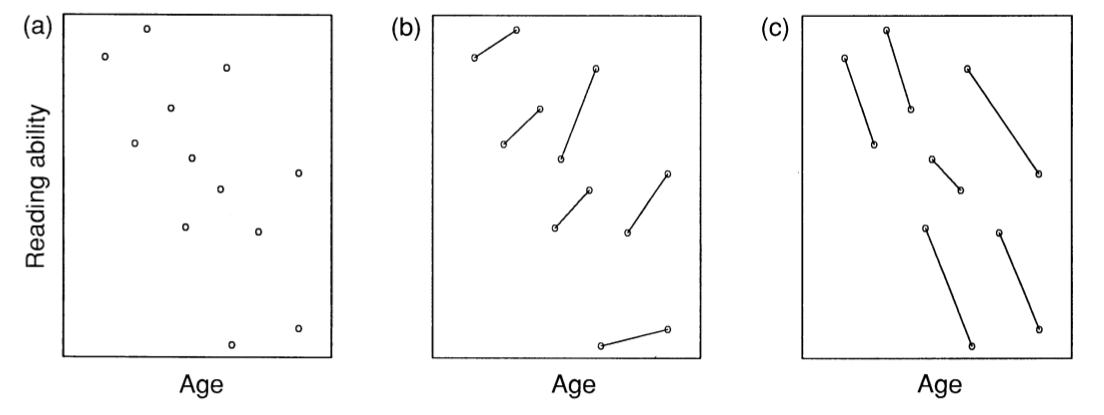
\includegraphics[width=.85\textwidth]{./Figs/Fig01.png}  
\end{figure}

\end{frame}


%%%%%%%%%%%%%%%%%%%%%%%%%%%%%%%%%%%%%%%%%%

\begin{frame}{Notation}

\bi
	\myitem We observe data $y_{ij}, \bx_{ij}$ for subjects $i = 1, \ldots I$ at visits $j = 1, \ldots, J_i$
	\myitem Vectors $\by_{i}$ and matrices $\bX_{i}$ are subject-specific outcomes and design matrices
	\myitem Total number of visits is $n = \sum_{i = 1}^{I} J_i$
	\myitem For subjects $i$, let
		$$ \by_{i} = \bX_{i} \bbeta + \bepsilon_{i}$$
	where $\var(\bepsilon_{i}) = \sigma^2 V_{i}$
\ei

\end{frame}


%%%%%%%%%%%%%%%%%%%%%%%%%%%%%%%%%%%%%%%%%%

\begin{frame}{Notation}

\bi
	\myitem Overall, we pose the model 
		$$ \by = \bX \bbeta + \bepsilon$$
	where $\var(\bepsilon) = \sigma^2 V$ and 
		$$ V = \left[ \begin{array}{cccc}
			V_1 		& 0 		& \ldots 	& 0 \\
			0 		& V_2	& \ldots 	& 0 \\
			\vdots 	& \vdots	& \ddots 	&  \\
			0 		& 0 		& 		& V_{I} \\
		 \end{array} \right]
		 $$
\ei


\end{frame}


%%%%%%%%%%%%%%%%%%%%%%%%%%%%%%%%%%%%%%%%%%

\begin{frame}{Covariates}

The covariates $\bx_{i} = x_{ij1} \ldots x_{ijp}$ can be
\bi
	\myitem Fixed at the subject level -- for instance, sex, race, fixed treatment effects
	\myitem Time varying -- age, BMI, smoking status, treatment in a cross-over design
\ei
\end{frame}


%%%%%%%%%%%%%%%%%%%%%%%%%%%%%%%%%%%%%%%%%%

\begin{frame}{Motivation}

Why bother with LDA?
\bi
	\myitem Correct inference
	\myitem More efficient estimation of shared effects
	\myitem Estimation of subject-level effects / correlation
	\myitem The ability to ``borrow strength" -- use both subject- and population-level information
\ei

\end{frame}


%%%%%%%%%%%%%%%%%%%%%%%%%%%%%%%%%%%%%%%%%%

\begin{frame}{Example dataset}

An example dataset comes from the Multicenter AIDS Cohort Study
\bi
	\myitem 366 HIV+ individuals
	\myitem Observation of CD4 cell count (a measure of disease progression)
	\myitem Between 1 and 11 observations per subject (1888 total observations)
\ei

\end{frame}


%%%%%%%%%%%%%%%%%%%%%%%%%%%%%%%%%%%%%%%%%%

\begin{frame}{Example dataset}

\begin{figure}[h]
    \includegraphics[width=.5\textwidth]{./Figs/Fig02.pdf}  
\end{figure}

\end{frame}


%%%%%%%%%%%%%%%%%%%%%%%%%%%%%%%%%%%%%%%%%%

\begin{frame}{Example dataset}

\begin{figure}[h]
    \includegraphics[width=.5\textwidth]{./Figs/Fig03.pdf}  
\end{figure}

\end{frame}


%%%%%%%%%%%%%%%%%%%%%%%%%%%%%%%%%%%%%%%%%%

\begin{frame}{Example dataset}

\begin{figure}[h]
    \includegraphics[width=.5\textwidth]{./Figs/Fig04.pdf}  
\end{figure}

\end{frame}


%%%%%%%%%%%%%%%%%%%%%%%%%%%%%%%%%%%%%%%%%%

\begin{frame}[t]{Visualizing covariances}

Suppose the data consists of three subjects with four data points each. 
\bi
	\myitem In the model
		$$ \by_{i} = \bX_{i} \bbeta + \bepsilon_{i}$$
	where $\var(\bepsilon_{i}) = \sigma^2 V_{i}$, what are some forms for $V_{i}$?
\ei

\end{frame}


%%%%%%%%%%%%%%%%%%%%%%%%%%%%%%%%%%%%%%%%%%

\begin{frame}{Approaches to LDA}

We'll consider two main approaches to LDA
\bi
	\myitem Random effects models, which introduce random subject effects (i.e. effects coming from a distribution, rather than from a ``true" parametric model)
	\myitem Marginal models, which focus on estimating the main effects and variance matrices but don't introduce subject effects
\ei

\end{frame}


%%%%%%%%%%%%%%%%%%%%%%%%%%%%%%%%%%%%%%%%%%

\begin{frame}{First problem: uniform correlation}

Start with the model where
$$V_{i} = \left[ \begin{array}{cccc}
			1 		& \rho	& \ldots 	& \rho \\
			\rho		& 1		& \ldots 	& \rho \\
			\vdots 	& \vdots	& \ddots 	&  \\
			\rho		& \rho	& 		& 1 \\
		 \end{array} \right]
$$
This implies 
\bi
	\myitem $var(y_{ij}) = \sigma^2$
	\myitem $cov(y_{ij}, y_{ij'})= \sigma^2 \rho$
	\myitem $cor(y_{ij},  y_{ij'})= \rho$
\ei

\end{frame}


%%%%%%%%%%%%%%%%%%%%%%%%%%%%%%%%%%%%%%%%%%

\begin{frame}{Random effects model}

A random intercept model with one covariate is given by 
$$ y_{ij} = \beta_{0} + b_{i} + \beta_{1} x_{ij} + \epsilon_{ij}$$
where
\bi
	\myitem $b_{i} \sim \N{0}{\tau^2}$
	\myitem $\epsilon_{ij} \sim \N{0}{\nu^2}$
\ei
Under this model
\bi
	\myitem $var(y_{ij}) = $
	\myitem $cov(y_{ij}, y_{ij'}) = $
	\myitem $cor(y_{ij},  y_{ij'}) = \rho = $
\ei

\end{frame}


%%%%%%%%%%%%%%%%%%%%%%%%%%%%%%%%%%%%%%%%%%

\begin{frame}{Marginal model}

The random intercept model is equivalent to the marginal model 
	$$ \by = \bX \bbeta + \bepsilon$$
where 
\bi
	\myitem $\var(\bepsilon) = \sigma^2 V$, 
	\myitem $$V_{i} = \left[ \begin{array}{cccc}
			1 		& \rho	& \ldots 	& \rho \\
			\rho		& 1		& \ldots 	& \rho \\
			\vdots 	& \vdots	& \ddots 	&  \\
			\rho		& \rho	& 		& 1 \\
		 \end{array} \right]
	$$
	\myitem $\sigma^2 = \tau^2 + \nu^2$
	\myitem $\rho = \frac{\tau^2}{\tau^2 + \nu^2}$
\ei

\end{frame}


%%%%%%%%%%%%%%%%%%%%%%%%%%%%%%%%%%%%%%%%%%

\begin{frame}{Partitioning variance}

\bi
	\myitem Whether we look at random effects or marginal modeling, we have to partition total variability into subject-level variance and population-level variance
	\myitem In a random effects framework, we estimate between and within subject variance components
	\myitem In a marginal model framework, we estimate a within subject variance and a covariance matrix
\ei

\end{frame}


%%%%%%%%%%%%%%%%%%%%%%%%%%%%%%%%%%%%%%%%%%

\begin{frame}[t]{Interpretation of ICC}

\bi
	\myitem The quantity $\rho = \frac{\tau^2}{\tau^2 + \nu^2}$ is called the intraclass correlation
	\myitem It tells how strongly observations within a subject are correlated relative to the overall population variance
	\myitem Alternatively, the ICC tells what proportion of variability is within-subject variability
\ei

\end{frame}


%%%%%%%%%%%%%%%%%%%%%%%%%%%%%%%%%%%%%%%%%%

\begin{frame}{Pig weight data}

\bi
	\myitem Weight on 48 pigs
	\myitem Nine measurements per pig
\ei

\end{frame}


%%%%%%%%%%%%%%%%%%%%%%%%%%%%%%%%%%%%%%%%%%

\begin{frame}{Pig weight data}

\begin{figure}[h]
    \includegraphics[width=.85\textwidth]{./Figs/Fig05.pdf}  
\end{figure}

\end{frame}


%%%%%%%%%%%%%%%%%%%%%%%%%%%%%%%%%%%%%%%%%%

\begin{frame}{Pig weight data}

\bi
	\myitem Apparent linear relationship
	\myitem High variance across pigs compared to variance within pigs
	\myitem Each pig's ``baseline" is vary important for future observations
\ei

\end{frame}


%%%%%%%%%%%%%%%%%%%%%%%%%%%%%%%%%%%%%%%%%%

\begin{frame}[fragile]{Pig weight data analysis}

Using ordinary least squares, we find 
\tiny
\begin{verbatim}
Coefficients:
            Estimate Std. Error t value Pr(>|t|)    
(Intercept) 19.35561    0.46054   42.03   <2e-16 ***
num.weeks    6.20990    0.08184   75.88   <2e-16 ***

Residual standard error: 4.392 on 430 degrees of freedom
\end{verbatim}

\end{frame}


%%%%%%%%%%%%%%%%%%%%%%%%%%%%%%%%%%%%%%%%%%

\begin{frame}{Pig weight data analysis}

\begin{figure}[h]
    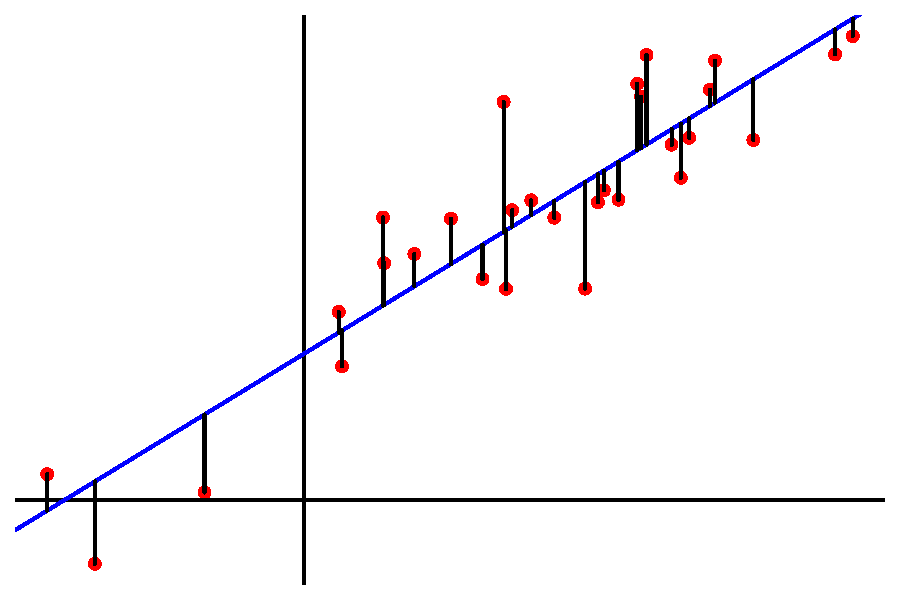
\includegraphics[width=.85\textwidth]{./Figs/Fig06.pdf}  
\end{figure}

\end{frame}


%%%%%%%%%%%%%%%%%%%%%%%%%%%%%%%%%%%%%%%%%%

\begin{frame}[fragile]{Pig weight data analysis}

Using a random intercept model, we find
\tiny
\begin{verbatim}
Random effects:
 Groups   Name        Variance Std.Dev.
 id.num   (Intercept) 15.1418  3.8913  
 Residual              4.3947  2.0964  
Number of obs: 432, groups: id.num, 48

Fixed effects:
            Estimate Std. Error t value
(Intercept) 19.35561    0.60311   32.09
num.weeks    6.20990    0.03906  158.97
\end{verbatim}

\end{frame}


%%%%%%%%%%%%%%%%%%%%%%%%%%%%%%%%%%%%%%%%%%

\begin{frame}{Pig weight data analysis}

\begin{figure}[h]
    \includegraphics[width=.85\textwidth]{./Figs/Fig07.pdf}  
\end{figure}

\end{frame}


%%%%%%%%%%%%%%%%%%%%%%%%%%%%%%%%%%%%%%%%%%

\begin{frame}{Next time}

\bi
	\myitem Why do we use random effects rather than creating subject-level indicator variables and estimating fixed effects?
	\myitem Next time we'll talk about estimation of random effect and marginal models
\ei

\end{frame}


%%%%%%%%%%%%%%%%%%%%%%%%%%%%%%%%%%%%%%%%%%

\begin{frame}{Today's big ideas}

\bi
	\myitem Longitudinal data analysis
	\myitem Uniform correlation models
\ei

\vspace{.75cm}
\hrule
\vspace{.75cm}

\end{frame}


%%%%%%%%%%%%%%%%%%%%%%%%%%%%%%%%%%%%%%%%%%
%%%%%%%%%%%%%%%%%%%%%%%%%%%%%%%%%%%%%%%%%%
%%%%%%%%%%%%%%%%%%%%%%%%%%%%%%%%%%%%%%%%%%

\end{document}

%%%%%%%%%%%%%%%%%%%%%%%%%%%%%%%%%%%%%%%%%%
%%%%%%%%%%%%%%%%%%%%%%%%%%%%%%%%%%%%%%%%%%
%%%%%%%%%%%%%%%%%%%%%%%%%%%%%%%%%%%%%%%%%%
%%%%%%%%%%%%%%%%%%%%%%%%%%%%%%%%%%%%%%%%%%
%%%%%%%%%%%%%%%%%%%%%%%%%%%%%%%%%%%%%%%%%%
%%%%%%%%%%%%%%%%%%%%%%%%%%%%%%%%%%%%%%%%%%